	
\documentclass[12pt]{article}
\usepackage{geometry} % see geometry.pdf on how to lay out the page. There's lots.
\geometry{a4paper} % or letter or a5paper or ... etc
% \geometry{landscape} % rotated page geometry
\usepackage{url}
\usepackage{graphicx}
\usepackage{placeins}
\usepackage{amsmath}
\usepackage[ruled,noend]{algorithm2e}
\usepackage[noend]{algorithmic}

\newcommand{\code}[1]{{\fontfamily{phv}\selectfont \small{\begin{tabbing} #1 \end{tabbing}}}}

\title{Natural Language Programming Analysis in Scala}
\author{\\ \'Eric Zbinden \\ \texttt{eric.zbinden@epfl.ch} \\ \\ Supervisors: \\Philippe Sutter(\texttt{philippe.sutter@epfl.ch})\\ Philipp Haller(\texttt{philipp.haller@epfl.ch})\\Prof. Viktor Kuncak(\texttt{viktor.kuncak@epfl.ch}) \\ \\ EPFL\\ Laboratory for Automated Reasoning and Analysis (LARA) \\ \url{http://lara.epfl.ch/}\\ Programming Methods Laboratory (LAMP) \\ \url{http://lamp.epfl.ch/} }
\date{\today}

\begin{document}

\maketitle
\newpage
\tableofcontents
\newpage

\section{Introduction}
...\\
For Java this was done by  

\section {Project Overview}
The main idea of this project is to apply an analysis similar to H{\o}st and {\O}stvold~\cite{DebugMN} but to Scala. Scala contains possibilities that Java don't contains; functional programming, local import. So I tried to focus on theses particularities as much as possible.

\section {Implementation}
The first thing is to retrieve information about a code. The best way is to create a plug-in for the Scala compiler. 

\subsection{Compiler plug-in}
My plug-in, named Scala-names, is inserted into the compiler phases right after phase 7:~\textit{refchecks}. It use the abstract syntax tree produced in previous phases to extract all objects named by the programmer. It could be variables names, objects names, methods names, parameters names or types names. It perform an analysis and then kill the resting compiler phases, as we don't need them.\\

By lack of time, the analysis is run only on method names. But the plug-in could easily be improved to also analyze other objects.
The plug-in check for every method definitions found in the given files and check if theses methods match features. See~\ref{features} for more details on features. The plug-in output for every methods found a list of "1" or "0" depending on this method satisfy or not a feature and the method name with source and position. See here an example of the output of the plug-in:
\code{1 1 0 0 0 0 1 1 0 0 0 0 0 0 0 1 1 0 0 1 0 0 0 0 1 0 0 0 0 0 0 0 0 1 0 0 0 0 0 \\empty@source-scala$\backslash$collection$\backslash$Map.scala,line-30,offset=1212}
You can see in the first line if the method, here \textit{empty} of the trait \textit{Map} defined in the \textit{scala$\backslash$collection$\backslash$Map.scala} file at line 30, match the features implemented inside the plug-in.
\subsection{Features}
\label{features}
A feature is a boolean property that a method may satisfy or not.\\
I tried to implement all the features that H{\o}st and {\O}stvold~\cite{DebugMN} used. I added features proper to the Scala language. Then I search into the \textit{Symbol} class given by the Scala compiler and implemented what I thought to be interesting and possible. Here is a list of features that I implemented:

\begin{enumerate}
\item ReturnTypeCOLLECTION :\\
	The return type is a collection. To be enough general to match a return of a List, a Set or a Map, it's implemented to match any class that extends the Traversable trait~\cite{travers}.
\item ReturnTypeOBJECT : \\
	This feature match any return type that extends the AnyRef class~\cite{anyRef}.
\item ReturnTypeUNIT :\\
	This feature match if the return type is Unit.
\item ReturnTypeBOOL : \label{fBool}\\
	Straight forward, this feature match boolean return type.
\item ReturnTypeINT :\label{fInt}\\
	Same as feature~\ref{fBool} with Integer return type.
\item ReturnTypeSTRING : \\
	Same as features~\ref{fBool} and~\ref{fInt} with String return type.
\item HasNoParameters :\label{fNoParam}\\
	This method is a variant of feature~\ref{fNoParenthesis}, see it for more details.
\item HasNoParenthesis :\label{fNoParenthesis}\\
In Scala when a programmer declare a function that take no argument, it's possible to write with or without parenthesis. With parenthesis indicate that this function have side effect; modifying data, printing out on std. In the AbstractSyntaxTree produced by the compiler, the parameters of a method are returned as a List of Lists. If the first list is empty, then it indicate that this method is declared without parameters and no parenthesis and should therefore have no side-effect. If the first list is of size one and contains an empty list, we have here a method declared without parameters but with parenthesis and thus with possible side-effect. And if the first list have a bigger size than one, it indicate we are dealing with a currified function.
\item ContainsIF :\\
	The method body contain an IF branch. Note that the Scala compiler translate WHILE block and DO-WHILE block with a IF branch. These two case should not match this feature as the programmer did not write any IF branch. IF guard statement in pattern matching are not taken in account as IF branch. However an IF branch inside a pattern matching right hand side will match. See here example of IF branch matching inside pattern matching right hand side:
\code{
ls \=match \{\\
\>case Nil =$>$\ false\\
\>case x\ ::\ xs =$>$\ if(x==0) true else false\\
\}
}
And IF guard inside pattern matching:
\code{
ls \=match \{\\
\>case Nil =$>$\ false\\
\>case x\ ::\ xs if(x==0) =$>$\ true\\
\>case x\ ::\ xs =$>$ false\\
\}
}
\item ContainsWHILE :\\
	The method body contains a WHILE statement. DO-WHILE statement are also considered as WHILE statement.
\item ContainsTRY-CATCH :\\
	The method body contains a TRY-CATCH block. If a method body contains only the TRY block, it will also match.
\item ContainsPatternMatching : \\
	The method body contains pattern matching. If match if the method body contains a MATCH statement.
\item ThrowException :\\
	The method body contains a THROW statement. It match only if it's explicitly declared. By example, A NumberFormatException raised by a wrong string applied to \textit{.toInt} will not match.
\item IsCurrified : \\
	This feature is a variant of feature~\ref{fNoParenthesis}.
\item IsSelfRecursif : \\
	This method call it-self in it's body. The feature don't match for other method even with surcharged identifiers. If a method call another method that call back the first method, it will not be considered as self-recursive.
\item MethodNameIsVerb : \label{fVerb}\\
	This feature match if the method name is a verb. It could be an infinitive or a conjugated form. For this feature, it use the WordNet 2.1 database~\cite{wordNet} to determine it.
\item MethodNameIsNoun :\\
	This feature match is the method name is a noun. As in feature~\ref{fVerb}, it use also the WordNet 2.1 database~\cite{wordNet}.
\item CamelPhrase : \label{fCamel}\\
	An unique word is not always meaningful to name a method. As C convention use underscore-separated words like "end\_of\_file", Java and Scala convention use camel case. Camel case is a practice of writing several words composed without white space but with the first letter of each word in uppercase. The first letter of the first word may or not be in uppercase.\\
This feature split the method name by the non-letter characters and by uppercase letters. Then it reconstruct potential acronym like in~\ref{fAcronym}. Then the feature will match if the split is composed at least of two words and if the second and followings words begin with an uppercase letter. Example:
\code{aCamel++Case\_PhraseWithXML \= =$>$ List(a, Camel, Case, Phrase, With, X, M, L)\\
\>=$>$ List(a, Camel, Case, Phrase, With, XML)\\
\>=$>$ true
}
Note that \textit{an\_Underscore\_Separated\_Phrase} will match this feature as all words, except the first, begin with an uppercase letter.
\item ContainsAcronym :\label{fAcronym}\\
	An acronym is defined by the aggregation of uppercase letter and digit. It must start with a letter. Non-letter nor digit characters are considered, as in feature~\ref{fCamel}, as blank and thus discarded. Inside a camel case phrase, the acronym is construct correctly: the acronym inside \textit{XMLAsString} is reconstruct as \textit{XML}. But as the underscore will also considered as a blank, two acronym separated by an underscore will create one acronym instead of two.\\
This feature will match if the method name contains at least one word that is an acronym.
\item MatchAbstractPhrase :\label{fAbstractPhrase} \\
	The method name is split the same manner as feature~\ref{fCamel} and if it contains the words \textit{get}, \textit{set}, \textit{contains} the next word should be a noun. If the method name contains the word \textit{is} it should be followed by an adjective. Like in feature~\ref{fContainsIs}, theses words can be written with a capital letter or without. If the method name don't contains theses four words, this feature return trivially true. This feature will also match on operators. See operators in feature~\ref{fOperator}.
\item ContainsWordIS :\label{fContainsIs}\\
	This feature match if the method name contains the word \textit{is}. \textit{is} can be written \textit{is} or \textit{Is}. As in features~\ref{fCamel} and~\ref{fAcronym}, the method name is split into words. Then if at least one word is \textit{is}, then the feature will match. 
\item ContainsWordGET :\label{fContainsGet}\\
	Straight forward, it's implemented the same way as feature~\ref{fContainsIs}.
\item ContainsWordSET :\label{fContainsSet}\\
	Same as features~\ref{fContainsIs} and~\ref{fContainsGet}.
\item ContainsWordCONTAINS :\label{fContainsContains}\\
	Same as features~\ref{fContainsIs},~\ref{fContainsGet} and~\ref{fContainsSet}.
\item IsValidJavaName :\label{fValidJavaName}\\
	A valid Java method name is a series of Java letters or Java digit that begin with a Java letter~\cite{jls_ident} and that is not a Java keyword~\cite{jls_keyword}. However the Scala library is developed in English, so for simplicity, it only take in count Latin characters without accent.
\item IsOperator :\label{fOperator}\\
	An operator is defined as a following of characters that are neither a letter neither a digit.
\item ReturnTypeCompletelyInMethodName :\label{fReturnTypeComplete}\\
	This feature match if the return type is contained into the method name. For composed return type name, the method name should match for every word of the return type. The return type name and the method name are split the same manner as in feature~\ref{fCamel}. 
\item ReturnTypePartiallyInMethodName :\\
	This feature is a variant of feature~\ref{fReturnTypeComplete}. For composed type name, as programmer are often lazy, they often write it partially. One would by example write only "Tree" instead of "AbstractSyntaxTree". This feature will match in such case as previous feature will not. It will also match if the type is completely contained, like~\ref{fReturnTypeComplete}.
\item RightAssociative :\\
	Scala language is left associative. But a method name that finish with the \textit{:} character is right associative.
%ajouter qqch ici
\code{
1\ ::\ List(2, 3) \==$>$ List(2, 3)::.(1)\\
\>=$>$ List(1, 2, 3)
}
This feature match if the last character of the method name is \textit{:}\ .
\item InnerMethod :\label{fInner}\\
	Scala language permit declaration of functions inside function. It's a good way to declare subroutine that should not be used outside of this function.\\
This feature match if the method body contains a method declaration.
\item ContainsInnerMethod :\\
	This feature is the opposite of feature~\ref{fInner} and match if the method body contains a method declaration.
\item Override : \\
	This feature match if this method override another method.
\item IsAbstract :\\
	This feature match if the method body is empty.
\item IsPublic  :\label{fPublic}\\
	A method declared public inside an object can be call within object. Note that inner function are always public but can't be accessed from outside.\\
This feature match if this method is public.
\item IsStatic :\\
	A static method can be called without having an object where the method is declared.\\
This feature match if this method is static. 
\item MethodNameFinishWithS :\label{fs}\\
	It's a naming convention that a method name finishing with a \textit{s} have a collection as return type.\\
This feature match if the last character of the method name is \textit{s}.
\item MethodNameFinishWithSS : \label{fss} \\
	Similar to feature~\ref{fs}, a method name finishing with \textit{ss} would mean this method return a collection of collections.\\ 
	This feature match if the two last characters of the method name are both~\textit{s}.
\item ContainsLazyVal :\\
	This feature match if the method body contains a lazy val.
\item IsImplicit : \\
	This feature match if the method is declared implicit.

\end{enumerate}
%See now an example of the plug-in applied on \textit{scala$\backslash$collection$\backslash$Map.scala} file.
%\code{
%1 1 0\=\ 0 0 0 1 1 0 0 0 0 0 0 0 1 1 0 0 1 0 0 0 0 1 0 0 0 0 0 0 0 0 1 0 0 0 0 0 \\\>empty@source-scala$\backslash$collection$\backslash$Map.scala,line-30,offset=1212\\
%0 1 0 0 0 0 1 1 0 0 0 0 0 0 0 0 0 1 0 1 0 0 0 0 1 0 1 1 0 0 0 0 0 1 1 0 0 0 1 \\\>canBuildFrom@source-scala$\backslash$collection$\backslash$Map.scala,line-46,offset=1551\\
%0 1 0 0 0 0 0 0 0 0 0 0 0 0 0 1 1 0 0 1 0 1 0 0 1 0 0 0 0 0 0 0 0 1 0 0 0 0 0 \\\>get@source-scala$\backslash$collection$\backslash$Map.scala,line-53,offset=1917\\
%0 1 0 0 0 0 1 1 0 0 0 0 0 0 0 0 0 0 0 1 0 0 0 0 1 0 1 1 0 0 0 0 0 1 0 0 0 0 0 \\\>iterator@source-scala$\backslash$collection$\backslash$Map.scala,line-54,offset=2020\\
%0 0 0 0 0 0 0 0 0 0 0 0 0 0 0 1 1 0 0 1 0 0 0 0 0 0 0 0 0 0 0 1 0 1 0 0 0 0 0 \\\>default@source-scala$\backslash$collection$\backslash$Map.scala,line-55,offset=2087\\
%1 1 0 0 0 0 1 1 0 0 0 0 0 0 0 0 0 0 0 1 0 0 0 0 1 0 0 0 0 0 0 1 0 1 0 0 0 0 0 \\\>seq@source-scala$\backslash$collection$\backslash$Map.scala,line-32,offset=1259\\
%1 1 0 0 0 0 1 1 0 0 0 0 0 0 0 1 1 0 0 1 0 0 0 0 1 0 0 0 0 0 0 0 0 1 1 0 0 0 0 \\\>empty@source-scala$\backslash$collection$\backslash$Map.scala,line-43,offset=1448\\
%0 0 0 0 1 0 1 1 0 0 0 0 0 0 0 1 1 0 0 1 0 0 0 0 1 0 0 0 0 0 0 1 0 1 0 0 0 0 0 \\\>size@source-scala$\backslash$collection$\backslash$Map.scala,line-52,offset=1872}
%Source code of \textit{empty@source-scala$\backslash$collection$\backslash$Map.scala,line-30,offset=1212}:\code{
%  def empty: Map[A, B] = Map.empty}
%\begin{itemize}1: the return type is a Map, and yes, it's a collection.\\
%Second feature is a 1: yes, Map is a subclass of AnyRef then yes. Third feature is a 0: Map is not Unit. Fourth feature is a 0: Map is not boolean.
%\end{itemize}
\subsection{Clustering}
\label{cluster}
With the output of the Scala-names plug-in, I filled the \textit{k}-means algorithm~\cite{kMeans} hoping the result will be interesting. The implementation of the algorithm follow~\cite{kMeans} description with a random partition. K-means is sensible to the initial partitioning and its output may be different. The output may also contains empty clusters. As k-means reach a stable point fast, It's generally recommended to run several time the algorithm to be sure to obtain a fine result.\\
First question, how many cluster should we use ? A too small number of clusters will aggregate different groups of methods and a too high number of clusters will separate methods in a same group. I think the answer to this question really depend on the data set and what we want to find. See~\ref{cluster:exp} for answer based on this project.\\
At the end of the algorithm, we obtain clustered data. Fine, but the center of cluster is a raw position, as it's the average position of all its members. To obtain a position more readable an more meaningful, I discrete the position of the clusters depending on a threshold to obtain a position only composed of: $0$, $1$ or $?$. If for a given dimension the value is lower than the threshold, the value is lowered to $0$. Respectively if the value is higher than $1-threshold$, the value is raised to $1$. And if the value is higher than the threshold and lower than $1-threshold$, the value is set to undefined: $?$. See figure~\ref{discrete} for an example on two dimensions.\\
Then I restart k-means with theses discrete clusters. During the project I was running only one-step of the algorithm, thinking it would not converge. This was at first to check the effect of the discretization to the clusters, but as it seams to converge, well take this advantage to get a better clustering. During this second run the distance to a cluster is defined this way:\begin{equation}\label{equa1}\mbox{if} (n-m ==0) \mbox{ Double.MAXVALUE else }\frac{n*d}{n-m}\end{equation} With $n$ the dimension of the cluster, $m$ the undefined values of this cluster and $d$ the distance calculate with defined values. Note that a completely undefined cluster would raise a division by zero and would learn us anything, thus it's distance is considered to be the maximum value to move members of this cluster to a more appropriate cluster. \\
Here, another question is raised: what's a relevant threshold ? It should be small enough to minimize the amount of methods that move to another cluster during the second k-mean run, but big enough to have a minimum of undefined values. See the respond in section~\ref{threshold}.
\begin{figure}[tbc]
\centering
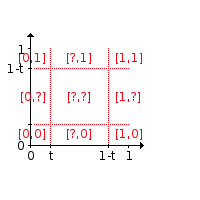
\includegraphics[width=5cm]{images/discrete.png}
\caption{Discretization of a cluster of two dimensions}
\label{discrete}
\end{figure}
\subsection{Analysis}
\label{analysis}
By giving the option "pAnalysis" to the plug-in, it's possible to analysis files compared to the Scala library. It's possible to pass several files with this option, but as the output of this option is quite long, it's recommended to pass only one file in argument. Like in previous points, it collect all method declarations. Then for every method declarations, it check all the 39 features and output a complete user friendly analysis. This analysis contains the signature of the method declaration, the nearest cluster of this declaration with it's distance, three methods from the Scala library took at random from the same cluster and for all features a line saying if this method declaration match the feature or not, referred to it's belonging cluster. If the method declaration is different to it's cluster, it will be noted. If the cluster is undefined for this feature, it output three dots. See an example of the output in annexes\ref{annexe1}.
\section {Experimental Results}

\subsection {Clustering}
\label{cluster:exp}
To answers the two questions of section~\ref{cluster}, I ran 100 times the k-means algorithm on the output of the Scala-names plug-in of the Scala library with different numbers of clusters. I took five mean metrics with confidence interval of 95\%: the number of empty clusters, the number of undefined values in all clusters, the average distance of methods to their respective cluster, the cluster average size and the error due to discretization modeled by the number of methods moving after a one-step of the second k-means. 
\subsubsection{Number of clusters}
For this series of experiments, the threshold was fixed at 0.15 . 
\\ \\
\begin{center}
\begin{tabular}{c c}
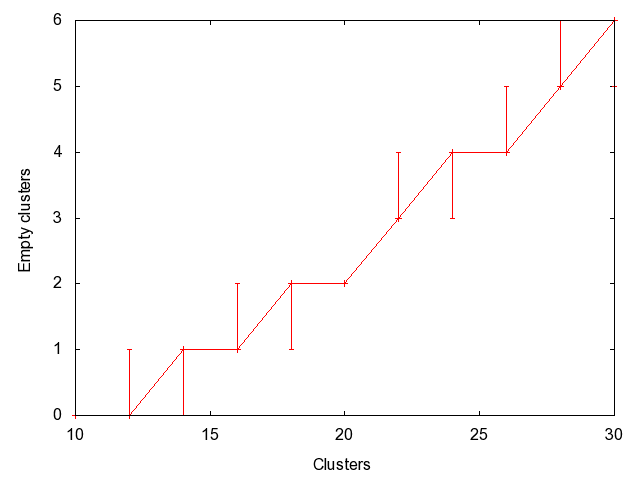
\includegraphics[width=5cm]{images/emptyCluster.png}
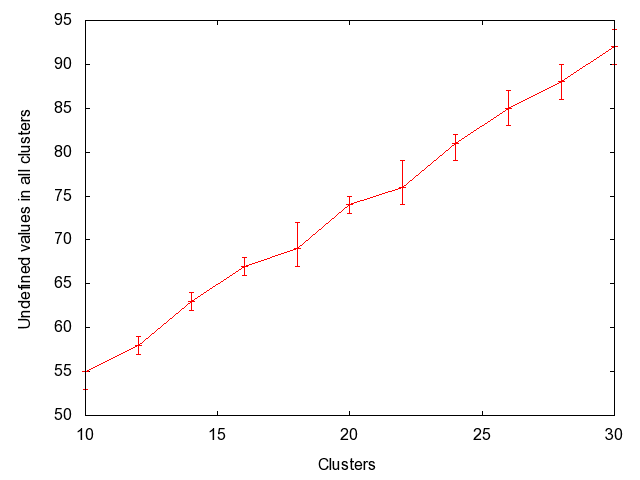
\includegraphics[width=5cm]{images/questionMark.png}
\end{tabular}\\
\begin{tabular}{c c c}
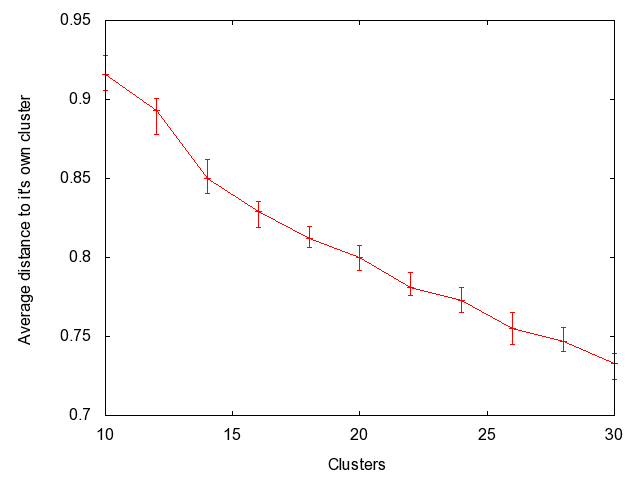
\includegraphics[width=5cm]{images/averageDist.png}
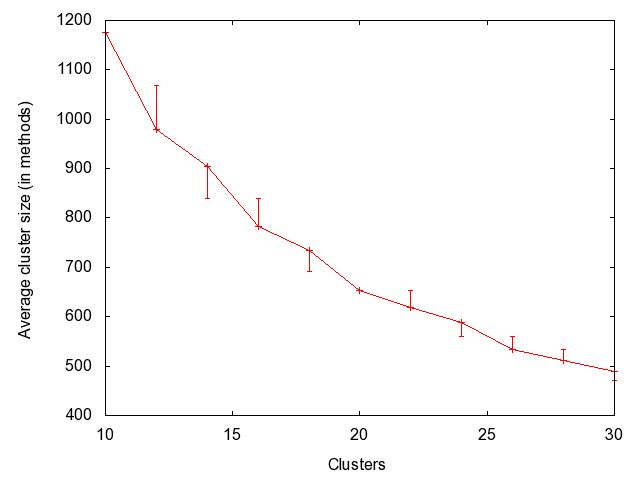
\includegraphics[width=5cm]{images/averageClusterSize.png}
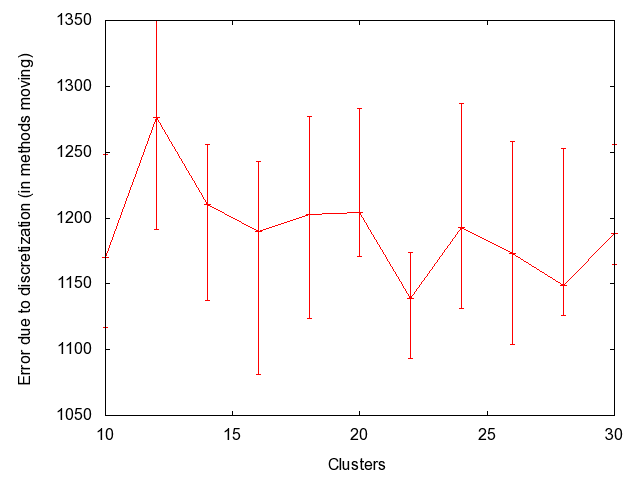
\includegraphics[width=5cm]{images/switched.png}
\end{tabular}
\end{center}

\begin{enumerate}
\item As the number of clusters increase, the number of empty clusters increase too. With fifty clusters we reach six empty clusters. It represent a percentage of empty cluster of 20\%, which is pretty high. There is no point to compute a clustering algorithm with a lot of clusters if they all finish empty. As The computational time of the algorithm also increase with a higher number of clusters, it suggest that a lower number of clusters is better.
\item To be independent of the first metric, the second it is calculated only with non-empty cluster. The number of undefined values in the clusters also increase with the cluster number on a linear basis. This is bad as we can't deduce anything from them. Again, it suggest a low number of clusters.
\item The third metric seams not really relevant. If the distance of a method to it's own cluster decrease, that's good, as the cluster is a better representation of its members. But as the result for ten cluster is already below a distance of one, a so small difference have no impact.
\item As the fourth metric show the average cluster size, we can pretend that a cluster with a smaller number of members will be more accurate. My experience on this project would say the same, as during the development of the project I get as a first result of k-means, with ten clusters, a pretty strange result. As all the ten clusters have a negative result for the pattern matching feature, I looked into some files at random, saw that it were true for those files and stated: "\textit{Yes, that's true, the Scala library do not contains any pattern matching.}" Off course, that's wrong. But pattern matching is found only in 8\% of all methods, making this feature less representative than feature with a higher probability. A small number of clusters will hide results on some features. On the other hand, as pointed by the second metric, the number of undefined values increase which try to say that to obtain a smaller granularity we need to cut some concentrated points.
\item The last metric seams unstable and really depend on the initial partitioning. But we need to consider the library size: 11'753 method declarations. The variation of the mean is of 1\% and the number of methods that move to another cluster stay on a percentage of 10\% of all methods. I noted that this percentage of moving methods was lower with a lower cluster dimension (i.e. less features). We can conclude that the number of clusters don't impact on the error due to discretization.
\end{enumerate}
On the basis of theses results, I decided to take a number of clusters of fifteen to shrink the cluster size at maximum without to suffer of bad effects of undefined values.
\subsubsection{Threshold}
\label{threshold}
Here again, I ran hundred times the same experience, but this time with a fixed number of clusters of fifteen, on different threshold. I choose the five same metrics. The number of empty clusters and the average cluster size are not represented here because they were constant. For every measures it return only one empty cluster and an average cluster size of 839,5 methods.
\begin{center}
\begin{tabular}{c c c}
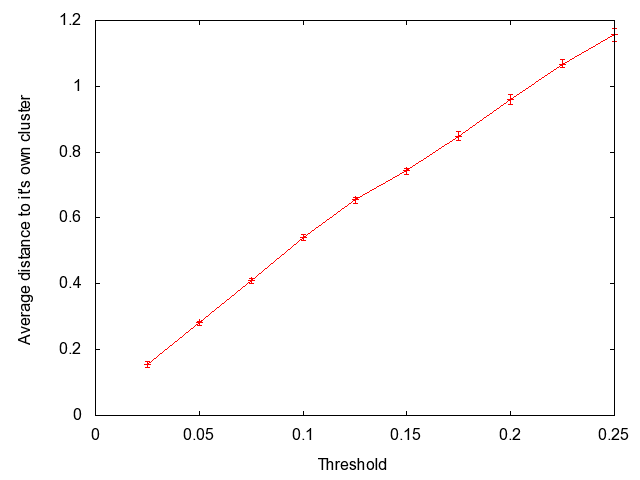
\includegraphics[width=5cm]{images/taverageDist.png}
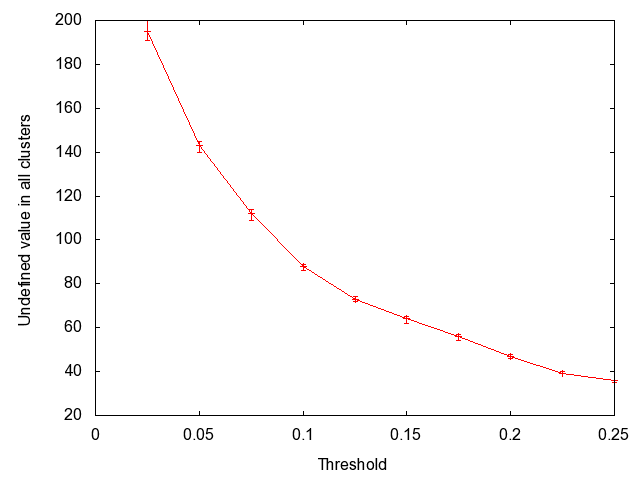
\includegraphics[width=5cm]{images/tquestionMark.png}
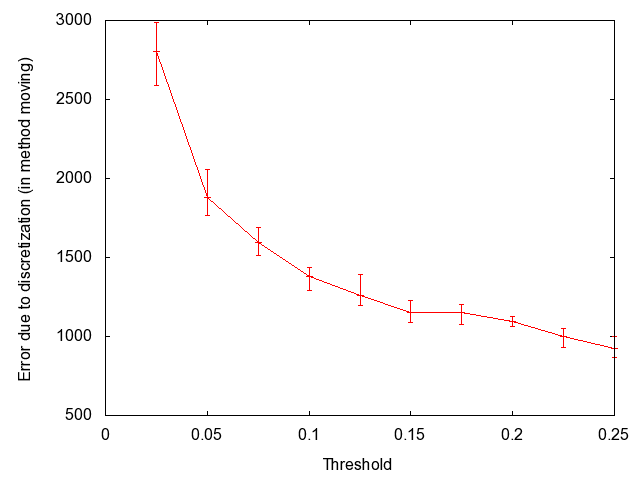
\includegraphics[width=5cm]{images/tswitch.png}
\end{tabular}
\end{center}
\begin{enumerate}
\item The average distance increase linearly with the threshold. The line cross a distance of 1 near a threshold of 0,2125. This distance depend on undefined values. For the same threshold, we have about 40 undefined values. So from equation~\ref{equa1} we can reconstruct the distance:\begin{align*}
1 &=\frac{n*d}{n-m}\\
d &= \frac{n-\frac{m}{c}}{n}
\end{align*} With $c$, the number of clusters fixed to 15 and $n$, the dimension of the clusters fixed to 39 (i.e. the number of features). We obtain:\begin{align}\label{equa2}
d = \frac{39-\frac{40}{15}}{39} = 0,9333
\end{align}

Equation~\ref{equa2} mean that the cluster represent correctly it's members with an error of one feature or an error of about $0,02$ per feature.\\ Note that I didn't test with a threshold of zero. I expected a such experience finishing with all clusters being filled only with undefined values.
\item As expected, the number of undefined values decrease as the threshold increase. This is a major criteria to obtain meaningful results.
\item The error due to discretization also decrease with the increase of the threshold. It's quite surprising. I was expecting an increase of the error with the threshold, as the greater the threshold is, the more the center of a cluster will be moved. This result come from the distance formula~\ref{equa1}, used to calculate the distance, that is greatly impacted by the number of undefined values. Let's see a concrete example or error of discretization:\\

Assume we use a threshold of 0,251 and two clusters of dimension five at respective position when k-means ends:\code{
cluster 1  = [1, 0.3, 0, 0, 0.75]\\
cluster 2 = [1, 0.4, 0, 0.5, 0.2]}
Now consider four methods, all belongs to cluster 1:
\code{method 1 = [1, 1, 0, 0, 1],\ \ \ \ \  $d_{c1}$ = 0.95,\ \ \ \ \  $d_{c2}$ = 1.9\\
method 2 = [1, 0, 0, 0, 0],\ \ \ \ \  $d_{c1}$ = 1.05,\ \ \ \ \  $d_{c2}$ = 1.1\\
method 3 = [1, 1, 0, 0, 1],\ \ \ \ \ $d_{c1}$ = 0.95,\ \ \ \ \  $d_{c2}$ = 1.9\\
method 4 = [1, 0, 0, 0, 1],\ \ \ \ \ $d_{c1}$ = 0.55,\ \ \ \ \  $d_{c2}$ = 1.7}
Now clusters become discrete: \code{
discrete cluster 1 = [1, ?, 0, 0, 1]\\
discrete cluster 2 = [1, ?, 0, ?, 0]}
Now compare the distance of the four methods to both clusters: \code{
 $d_{m1-c1}$ = 0,\ \ \ \ \ \ \ \ \ $d_{m1-c2}$ = 2.25\\
$d_{m2-c1}$ = 1.25, \ \ \ $d_{m2-c2}$ = 0\\
$d_{m3-c1}$ = 0,\ \ \ \ \ \ \ \ \ $d_{m3-c2}$ = 2.25\\
$d_{m4-c1}$ = 0,\ \ \ \ \ \ \ \ \ $d_{m4-c2}$ = 1.25}
The method 1, 3 and 4 will stay inside cluster 1. But method 2 will move to cluster 2. As the distance is only calculated with defined values, methods will be closer to clusters that have no difference with them on the defined values. At the opposite, a difference will obtain a bigger impact. The number of undefined value also affect the distance as a factor.
\end{enumerate}
We can ask our-self what would happen if we run k-mean algorithm directly with discrete clusters. As k-mean is impacted by the random partitioning, I make the assumption that the algorithm would not work properly and end with all cluster with all dimensions undefined. And would k-mean with discrete cluster converge after the end of k-mean with continuous position ? I was assuming it won't, but I tried several times and it seams that it always converge. Note it would need a bigger number of trials to really prove that it always converge.\\
On the basis of theres results, a threshold of 0,2125 seams the most appropriate. It's a high threshold and the distance of methods to their own cluster stay correct.

\subsection {Features}
\begin{figure}
\centering
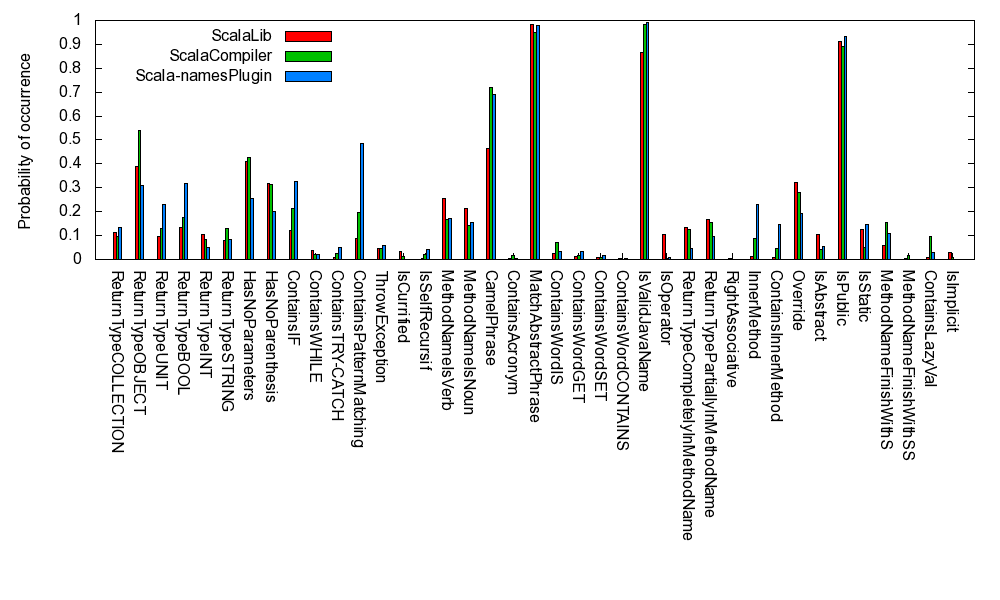
\includegraphics[width=15cm]{images/percent.png}
\caption{Probabilities of occurrence of features.}
\label{fig:features}
\end{figure}
In figure~\ref{fig:features} we can see the probability of occurrence of all 39 features inside the Scala library, the Scala compiler and in the Scala-names plug-in. Note that the package \textit{scala$\backslash$tools$\backslash$ant} of the Scala compiler is not contained inside this analysis. This represent 11'753 method declarations inside the Scala library, 11'730 in the Scala compiler and 199 for the Scala-names plug-in. We can note from figure~\ref{fig:features} that I use a lot more of pattern matching in this project than it's used inside the Scala library or compiler. The library and the compiler also contains less inner methods. We can argue from theses facts that the Scala library and compiler are written in a better Scala-way of coding.
\begin{enumerate}
%\item Feature~\ref{fCollection} and~\ref{fs} should be correlated as it's a convention that method returning a collection finish with \textit{s}. The correlation matrix in figure~\ref{corrCor} output a 0.8
\item The feature~\ref{fss} reveal to be absolutely useless. I checked manually all method declared inside the Scala library, all methods matching this feature are composed of word that finish with two \textit{s} like: \textit{access, success} or \textit{Class}. They are not declared with \textit{ss} because their return type are a collection of collections, but because theses words take two \textit{s}. I was so disappointed that I didn't even implemented a feature that check a return type of collection of collections, thinking that it would be a waste of time. Note that maybe some methods are actually of this return type. 
\end{enumerate}
\subsubsection {Correlation}
Figures~\ref{corrCor} and~\ref{corrCor2} show the correlation between two features in the Scala library and respectively in the Scala compiler. The correlation is calculated as follow: for every method definitions inside the corpus, for every features two by two, addition the number of time both features are equals and divide the result by the number of method definitions in the corpus. If two features are often both found or both negative in a single method definition, they have a high correlation coefficient. Note that this does not mean that they are really correlated. By example, if no plane crash today and no nuclear power plant explode today, this doesn't mean that tomorrow if a plane crash, the nearest nuclear power plant will explode. Thanks Philippe for this example.\\
Figures~\ref{corrJac} and~\ref{corrJac2} show the Jaccard coefficient. It measures the similarity between two features respectively in the Scala library and in the Scala compiler. It's calculated as follow: for every method definitions inside the corpus, for every features two by two, addition the number of time both feature are equals to one and divide the result by the amount of methods definitions.
\begin{figure}[h]
\centering
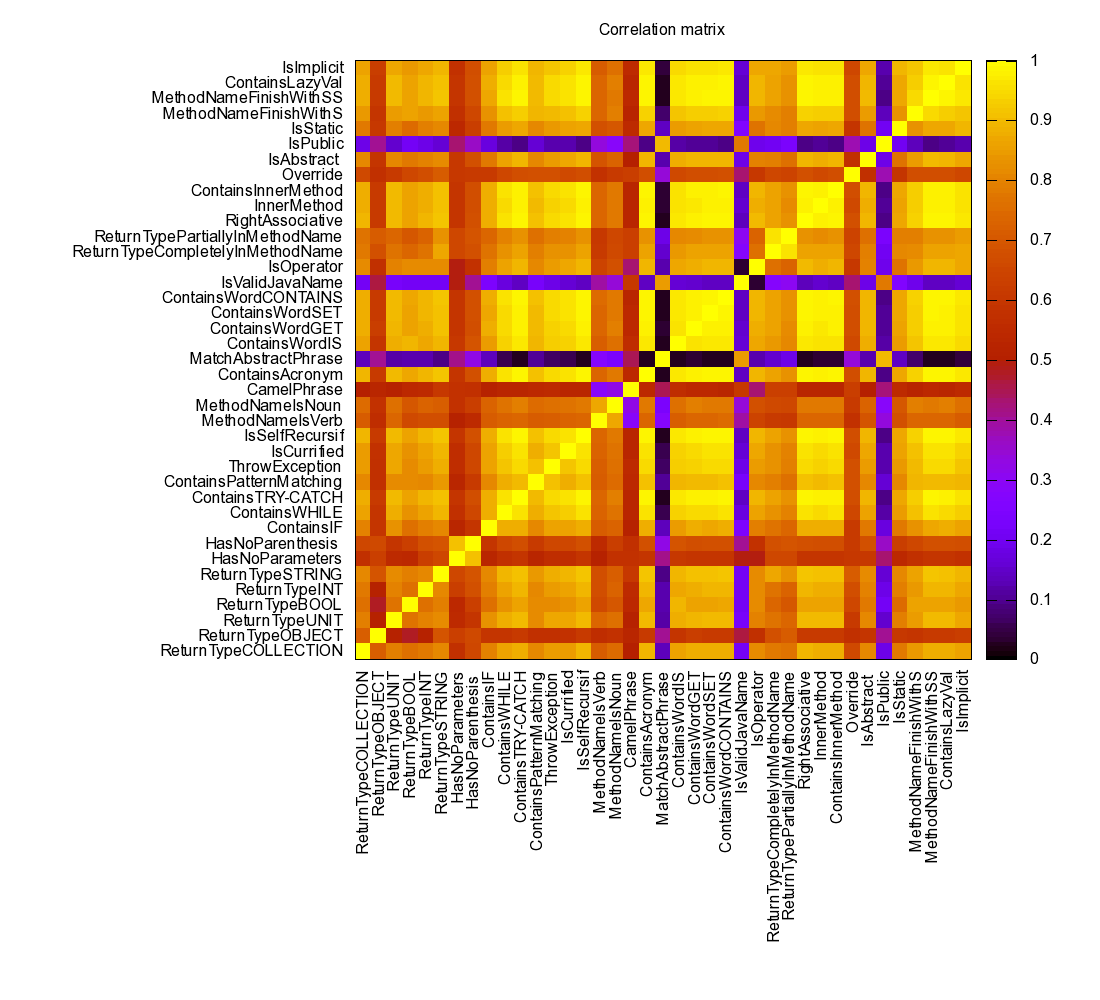
\includegraphics[width=17cm]{images/corrCOR.png}
\caption{Correlation matrix in Scala library}
\label{corrCor}
\end{figure}
\begin{figure}[h]
\centering
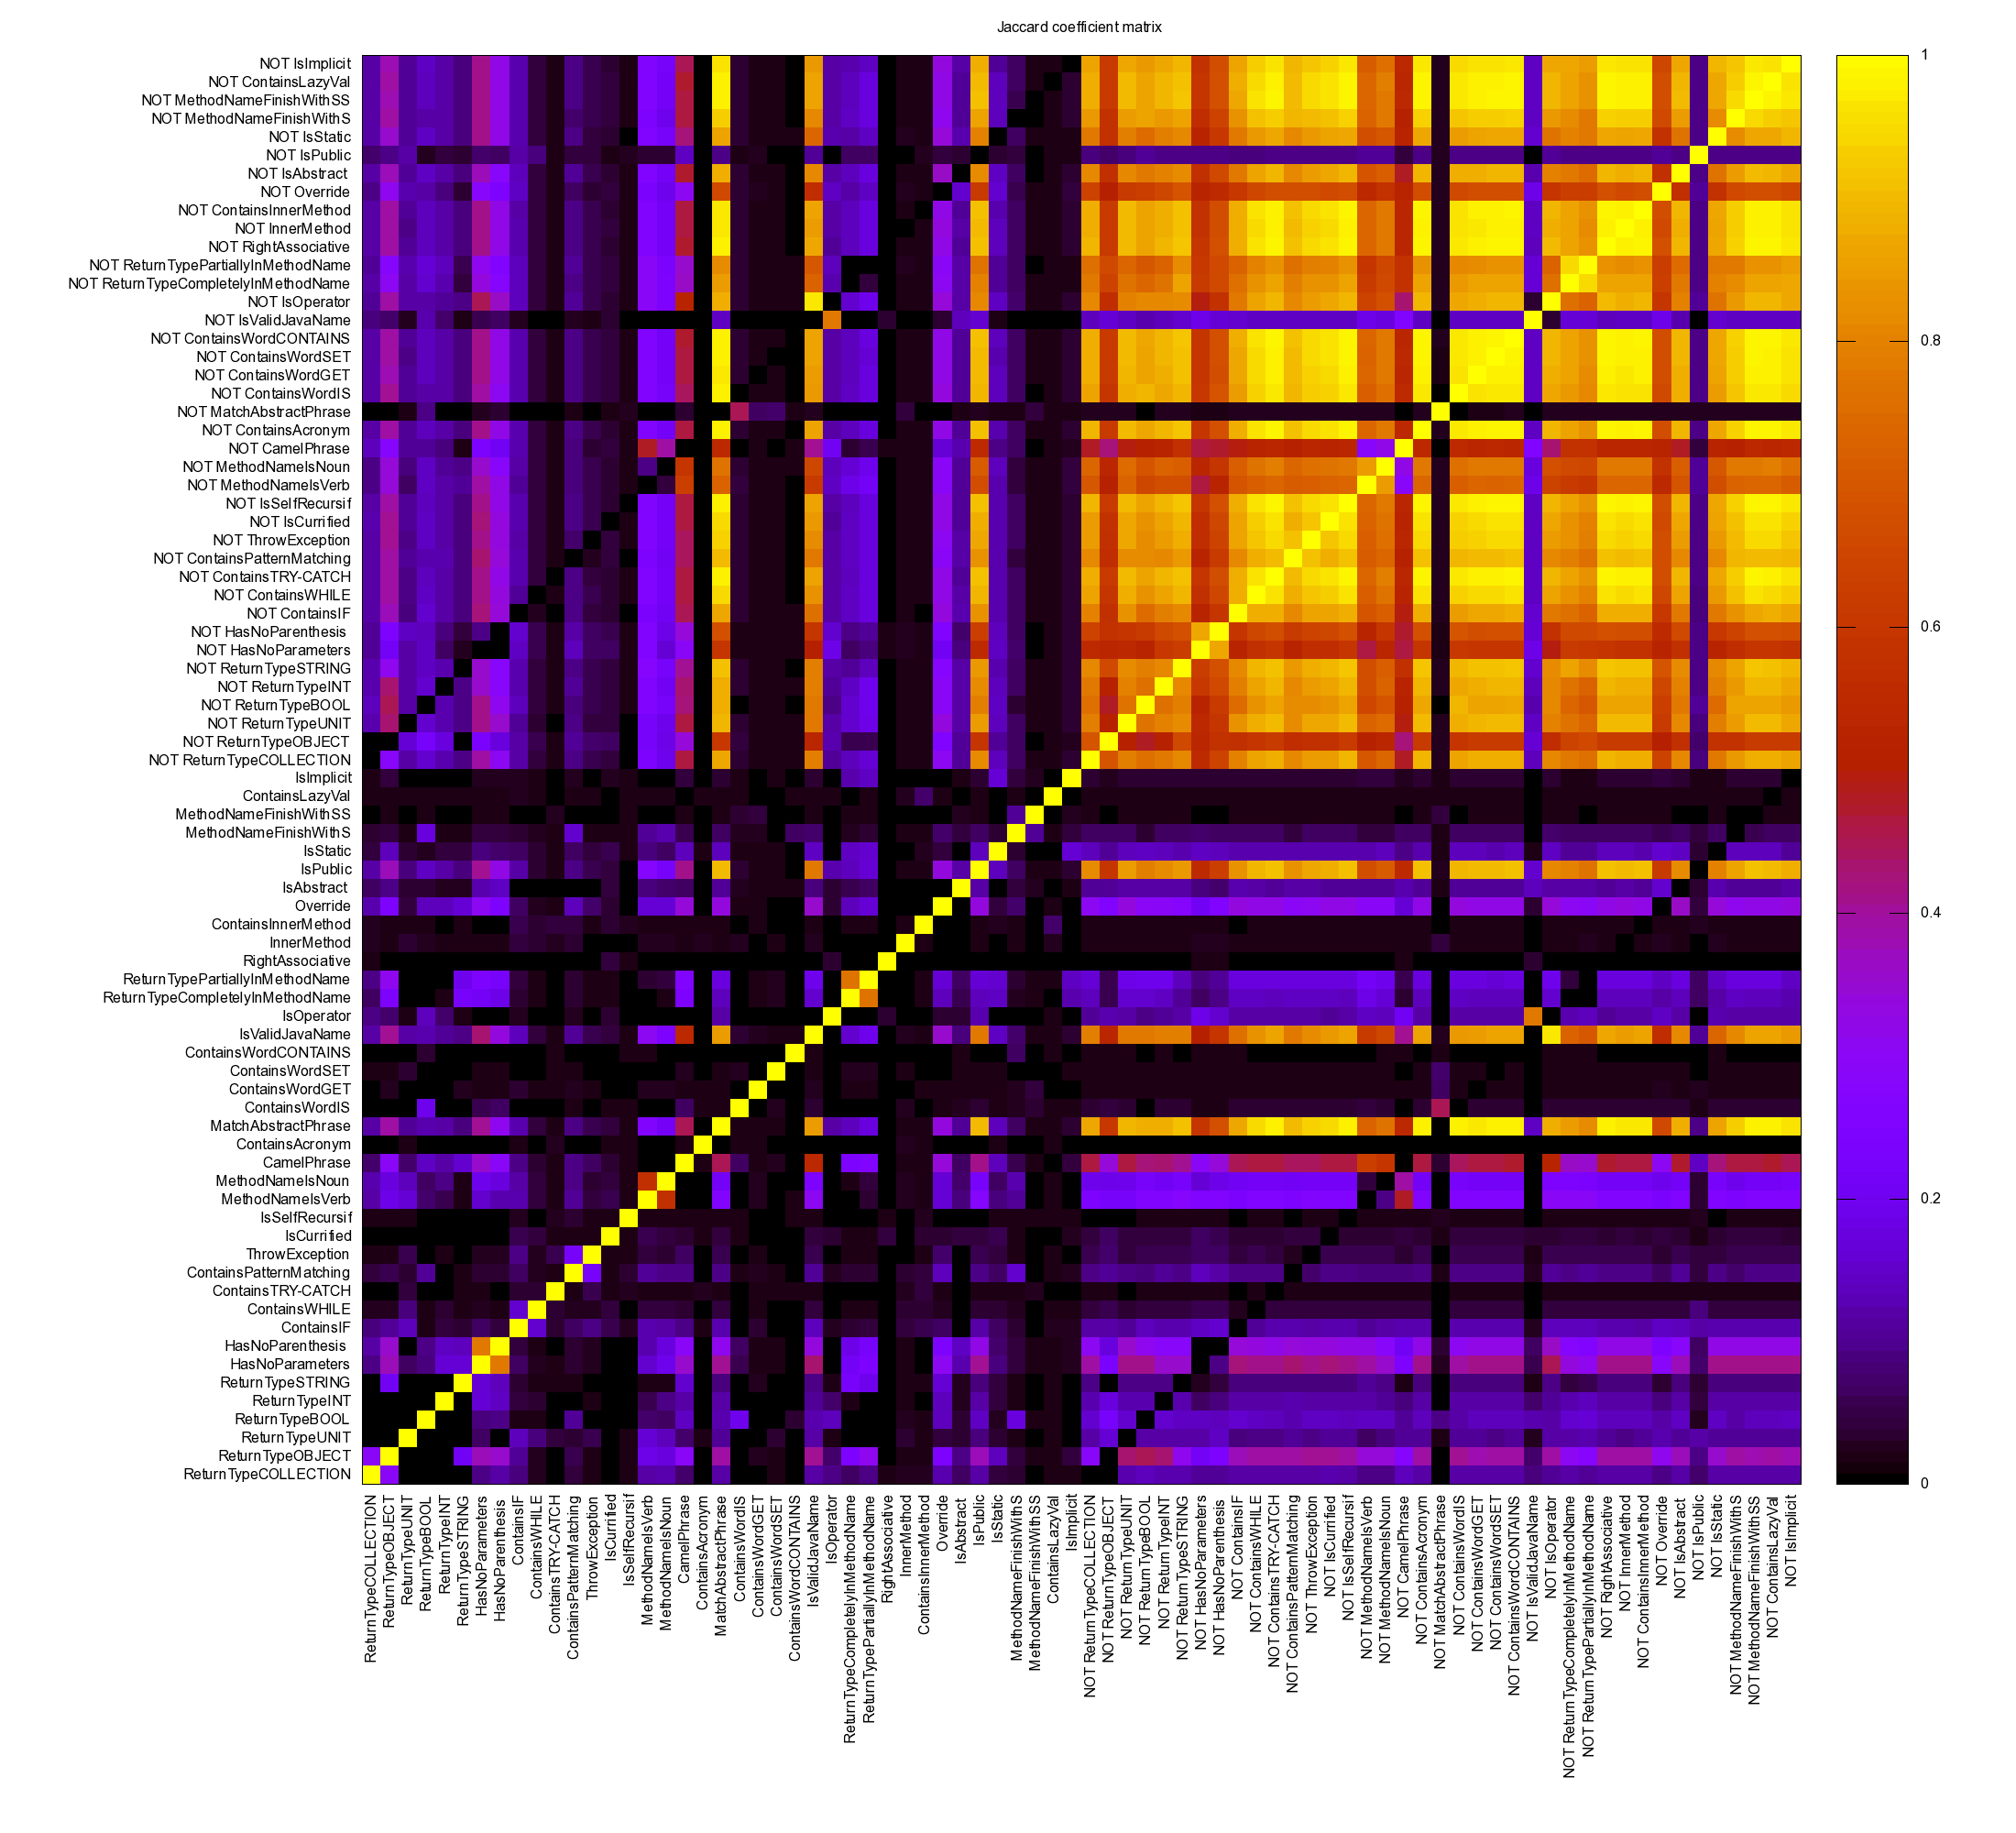
\includegraphics[width=17cm]{images/corrJAC.png}
\caption{Jaccard coefficient matrix in Scala library}
\label{corrJac}
\end{figure}
\begin{figure}[h]
\centering
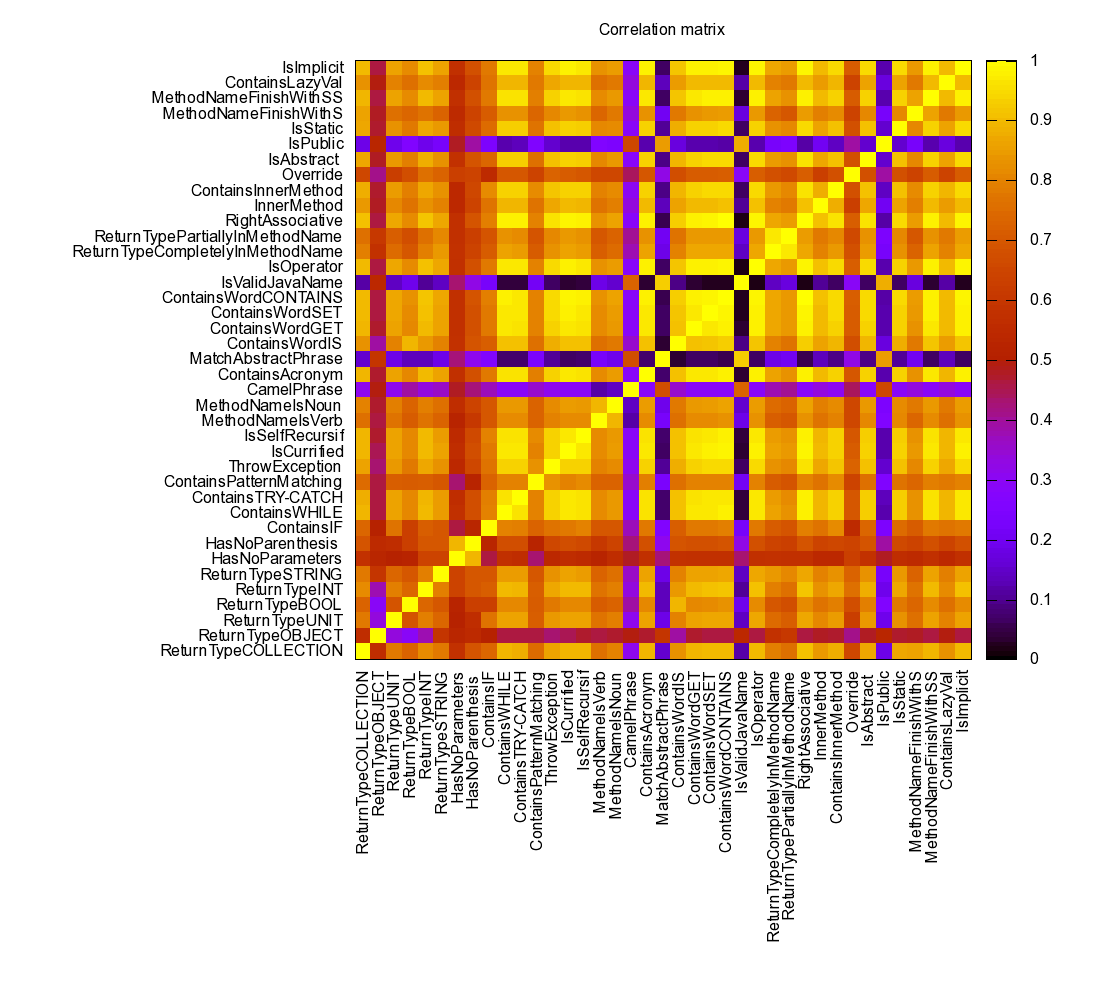
\includegraphics[width=17cm]{images/corrCOR2.png}
\caption{Correlation matrix in Scala compiler}
\label{corrCor2}
\end{figure}
\begin{figure}[h]
\centering
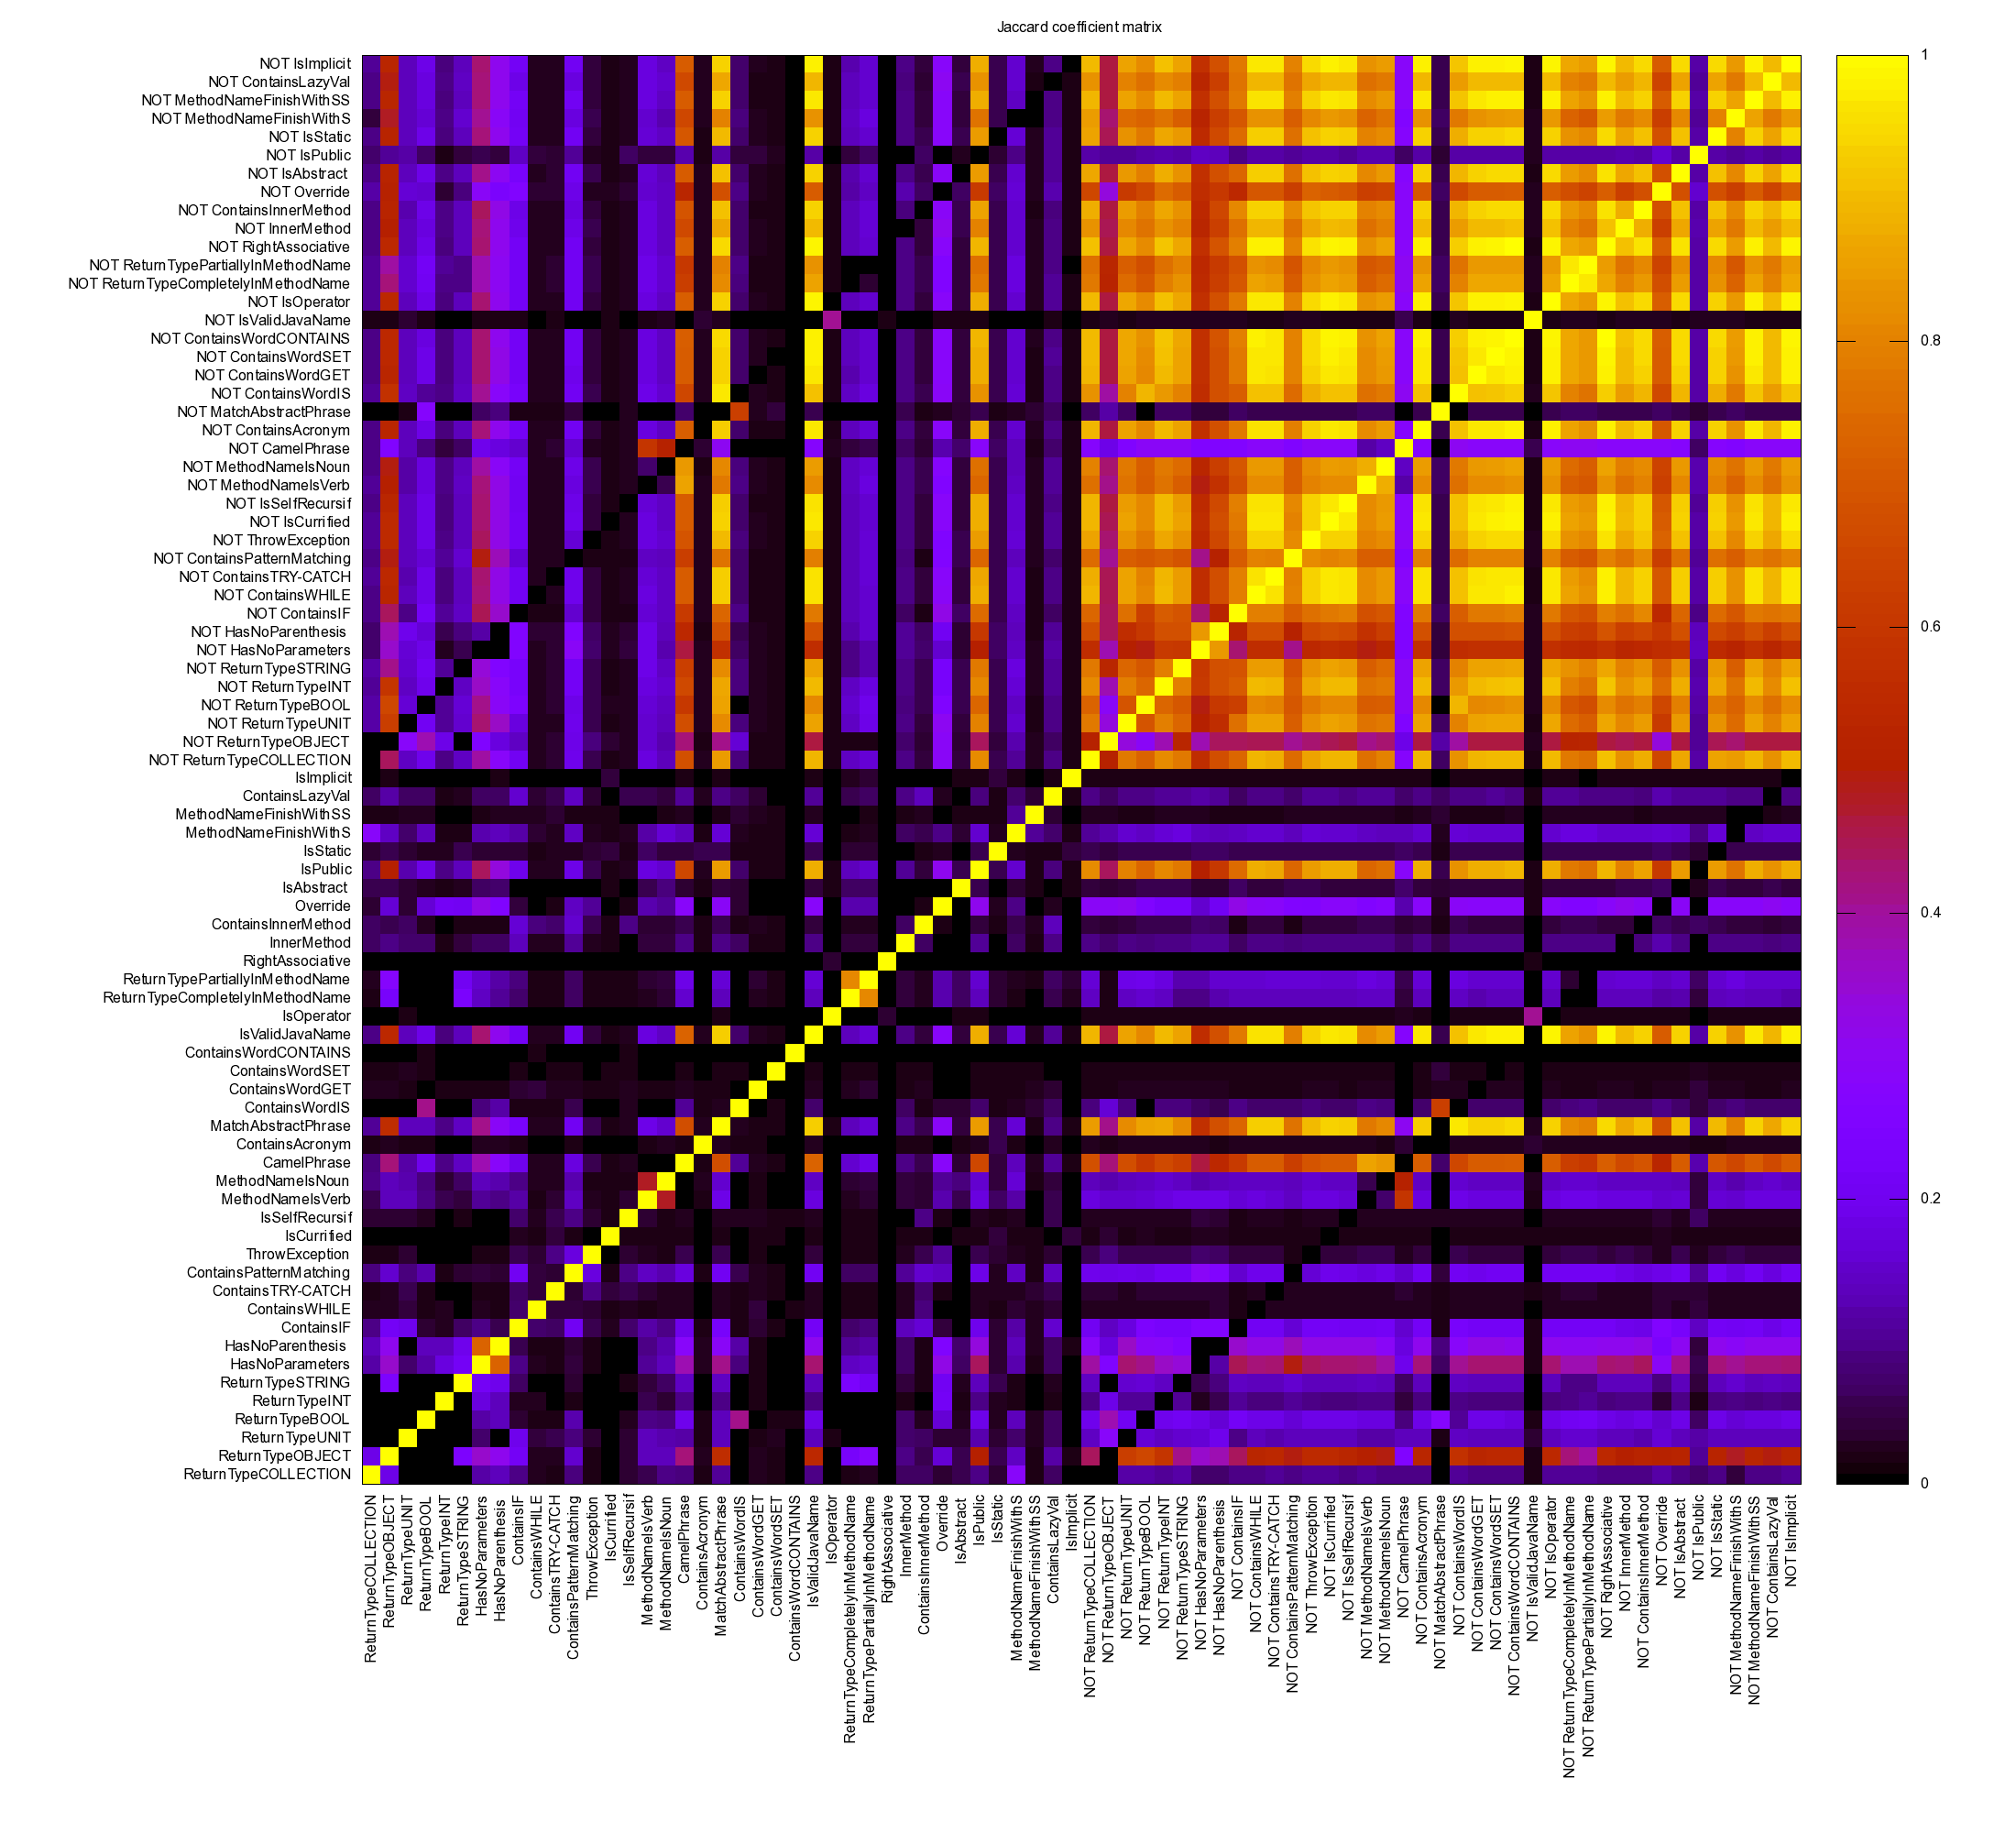
\includegraphics[width=17cm]{images/corrJAC2.png}
\caption{Jaccard coefficient matrix in Scala compiler}
\label{corrJac2}
\end{figure}
\FloatBarrier
\begin{enumerate}
\item The first thing we see in correlation matrix of figure~\ref{corrCor} is these three blue-black lines. The three features~\ref{fAbstractPhrase},~\ref{fValidJavaName} and~\ref{fPublic} at theses lines are the three more likely feature to appear. As compared to theses others features appear not so often, their correlation coefficient is really low.
\item Features~\ref{fContainsIs},~\ref{fContainsGet},~\ref{fContainsSet} and~\ref{fContainsContains} are highly correlated. Of theses features, the~\ref{fContainsIs} is the more present with 2\%, the others are present in less than 1\%. This correlation become from the fact that theses features are very unlikely, they are nearly every times negative and thus are near all the time identical. Others features with a probability lower than 1\% obtain a high correlation with theses four features for the same reason. Note that in the correlation matrix of Scala compiler, figure~\ref{corrCor2}, the correlation of feature \textit{ContainsIS}~\ref{fContainsIs} is a bit lower. It's because this feature is more likely to happen, with a 7\%.\\I choose theses four words to be features as they are very often used in Java programming. But it clearly seams it's not the case in Scala. It may be interesting to try a similar feature with \textit{apply}. 
\item Note the difference of color between figure~\ref{corrCor} and~\ref{corrCor2}. The correlation matrix of the Scala compiler is slightly darker. This come from the fact that a good number of features are more present in the Scala compiler methods than in Scala library. We found out an inverse result on the color of figures~\ref{corrJac} and~\ref{corrJac2}. Colors of some dots are more warmer. This is the result of the same fact.
\end{enumerate}

\section {Conclusion} 
To obtains better results, feature with a higher probability are better.

\section {Future and Related Work}
%Add new features, look at object, trait and class. Parameters and variables. 
\subsection{Adding New Features}
The list of features implemented is off course not exhaustive and can be improved. Here is a list of possible interesting features:
\begin{itemize}
\item The Scala compiler can infer type. So programmers don't need to always specify the return type of a method. In some case the type could be a good indication to the reader to understand the code. But in other case like the method \textit{toString()} we don't really need to see the type written to know its type. Adding a feature returning if the type is declared or inferred, may obtain information about code quality.
\item A feature matching assignment of variables declared in a larger scope.
\end{itemize}
\subsection{Compose With Others Analysis}
Method name are not the only "object" that the programmer name. He also name variables, class, parameters and types. An analysis of these "objects" can also find out to be interesting. By example, the feature~\ref{fss} give nothing with method name but could highlight something on variables.\\
Cross analysis on all objects can also demonstrate some results.\\
%ajouter ce que Jd m'a parlé

\newpage
\section{Annexes}
\subsection{Analysis example}
\label{annexe1}
This is an example of the analysis output for one method described in section~\ref{analysis}. When you analyze a file you will get a similar output for every method declarations in that file.\code{
--- Method: splitAt@source-.$\backslash$scala$\backslash$collection$\backslash$immutable$\backslash$List.scala,line-191,offset=6483 ---\\
Sign: 0 1 0 0 0 0 0 0 0 1 0 0 0 0 0 0 0 1 0 1 0 0 0 0 1 0 0 0 0 0 0 1 0 1 0 0 0\\
Nearest cluster: 8 at distance 2.0097560975609756\\
cPos: 0 0 0 ? ? 0 ? 0 0 0 0 ? ? 0 0 0 0 1 0 1 0 0 0 0 1 0 0 0 0 0 0 1 0 1 0 0 0\\
Similar methods:\\
\ \ \ \ \ \ \ \ \ hashCode@source-.$\backslash$scala$\backslash$concurrent$\backslash$pilib.scala,line-127,offset=3904\\
sign: 0 0 0 0 1 0 1 0 0 0 0 0 0 0 0 0 0 1 0 1 0 0 0 0 1 0 0 0 0 0 0 1 0 1 0 0 0\\
\ \ \ \ \ \ \ \ \ canEqual@source-.$\backslash$scala$\backslash$Option.scala,line-261,offset=9053\\
sign: 0 0 0 1 0 0 0 0 0 0 0 0 0 0 0 0 0 1 0 1 0 0 0 0 1 0 0 0 0 0 0 1 0 1 0 0 0\\
\ \ \ \ \ \ \ \ \ productElement@source-.$\backslash$scala$\backslash$reflect$\backslash$generic$\backslash$Trees.scala,line-190,offset=6295\\
sign: 0 0 0 0 0 0 0 0 0 0 0 1 1 0 0 0 0 1 0 1 0 0 0 0 1 0 0 0 0 0 0 1 0 1 0 0 0\\
Haz NOT\ \ \ \ \ \ \ \ \ \ \ \ \ \ \ \ \ \ \ \ \ \ \ \ \ \ \ \ \ \=Method returns a collection (Traversable).\\
Haz \ \ \ \ \ \ \ \ BUT should NOT Method returns a subtype of class Object.\\
Haz NOT                \>Method return is of type: class Unit.\\
Haz NOT\ \ \ \ \ \ \ \ \ \ \ \ \ ...       \>Method return is of type: class Boolean.\\
Haz NOT\ \ \ \ \ \ \ \ \ \ \ \ \ ...       \>Method return is of type: class Int.\\
Haz NOT                \>Method return is of type: class String.\\
Haz NOT\ \ \ \ \ \ \ \ \ \ \ \ \     ...       \>Method have no parameter.\\
Haz NOT                \>Method has no parenthesis.\\
Haz NOT                \>Method contains IF statement.\\
Haz \ \ \ \ \ \ \ \ BUT should NOT Method contains WHILE statement.\\
Haz NOT                \>Method contains TRY/CATCH statement.\\
Haz NOT\ \ \ \ \ \ \ \ \ \ \ \ \ ...       \>Method contains Pattern matching.\\
Haz NOT\ \ \ \ \ \ \ \ \ \ \ \ \ ...       \>Method may explicitly throw an exception.\\
Haz NOT                \>Method is currified.\\
Haz NOT               \> Method contains a self-recursion.\\
Haz NOT               \> Method name is a verb\\
Haz NOT               \> MethodName is a noun\\
Haz  \ \ \ \ \ \ \                    \> Method name is a camel phrase.\\
Haz NOT               \> Method name contains an acronym\\
Haz  \ \ \ \ \ \ \                   \> Method name match abstract phrase construction.\\
Haz NOT               \> MethodName contains "is" pattern.\\
Haz NOT                \>MethodName contains "get" pattern.\\
Haz NOT               \> MethodName contains "set" pattern.\\
Haz NOT               \> MethodName contains "contains" pattern.\\
Haz  \ \ \ \ \ \ \                   \> MethodName is a valid Java name.\\
Haz NOT               \> MethodName is an operator\\
Haz NOT               \> Method return type is completely contained into methodName. \\
Haz NOT\>Method return type is partially into the method name\\
Haz NOT               \> This method is right associative\\
Haz NOT\>This method is defined inside another method\\
Haz NOT               \> Method body contains method definition\\
Haz  \ \ \ \ \ \ \           \>         Method is overriding another method\\
Haz NOT        \>        This Method is abstract\\
Haz  \ \ \ \ \ \ \            \>        This method is public\\
Haz NOT             \>   This method is static\\
Haz NOT\>This method finish with s\\
Haz NOT           \>     This method finish with ss}


\newpage

\bibliographystyle{plain}
\bibliography{EricZbinden_ScalaNames}

\end{document}